\documentclass{beamer}
\usepackage{graphicx}
\usepackage{blindtext}
\usepackage{natbib}
\mode<presentation> {
\usetheme{Warsaw}
\usecolortheme{crane}}
\title{I social e il populismo}
\author{Alessandro Meloni, Alessandro Casanova}
\date{16/11/2023}

\begin{document}
\maketitle
 
\begin{frame}{Presentazione}
    \centering
    Although frequently used by historians, social scientists, and political commentators, the term [populism] is exceptionally vague and refers in different contexts to a bewildering variety of phenomena (Margaret Canovan).\\
    A thin-centred ideology that considers society to be ultimately separated into two homogenous and antagonistic camps, "the pure people" versus "the corrupt elite", and which argues that politics should be an expression of the volonté générale (general will) of the people (Mudde and Rovira Kaltwasser).
\end{frame}
\begin{frame}
    Populism here becomes a catch-all label to refer to all those political phenomena that are considered to be dangerous, irrational and demagogic; populism as a politics that appeals to the basest sentiments of the populace, makes demagogic promises and panders to imaginary fears.
    \citep{Gerbaudo2018}

\end{frame}
\begin{frame}{Cos'è il Populismo?}
\begin{itemize}
    \item Nasce in America e in Russia
    \item Presenta idee agrarie, progressiste e il "popolo" come virtuoso ma schiavo delle autorità
    \item Propone idee "semplici" e immediate per risolvere i problemi
    \item Crea l'immagine di un leader che guida, spesso utilizzando stereotipi sul suo carattere
    \item Immagina un mondo diviso tra "noi" e "loro"
\end{itemize}
\end{frame}

\begin{frame}
    \flushleft
    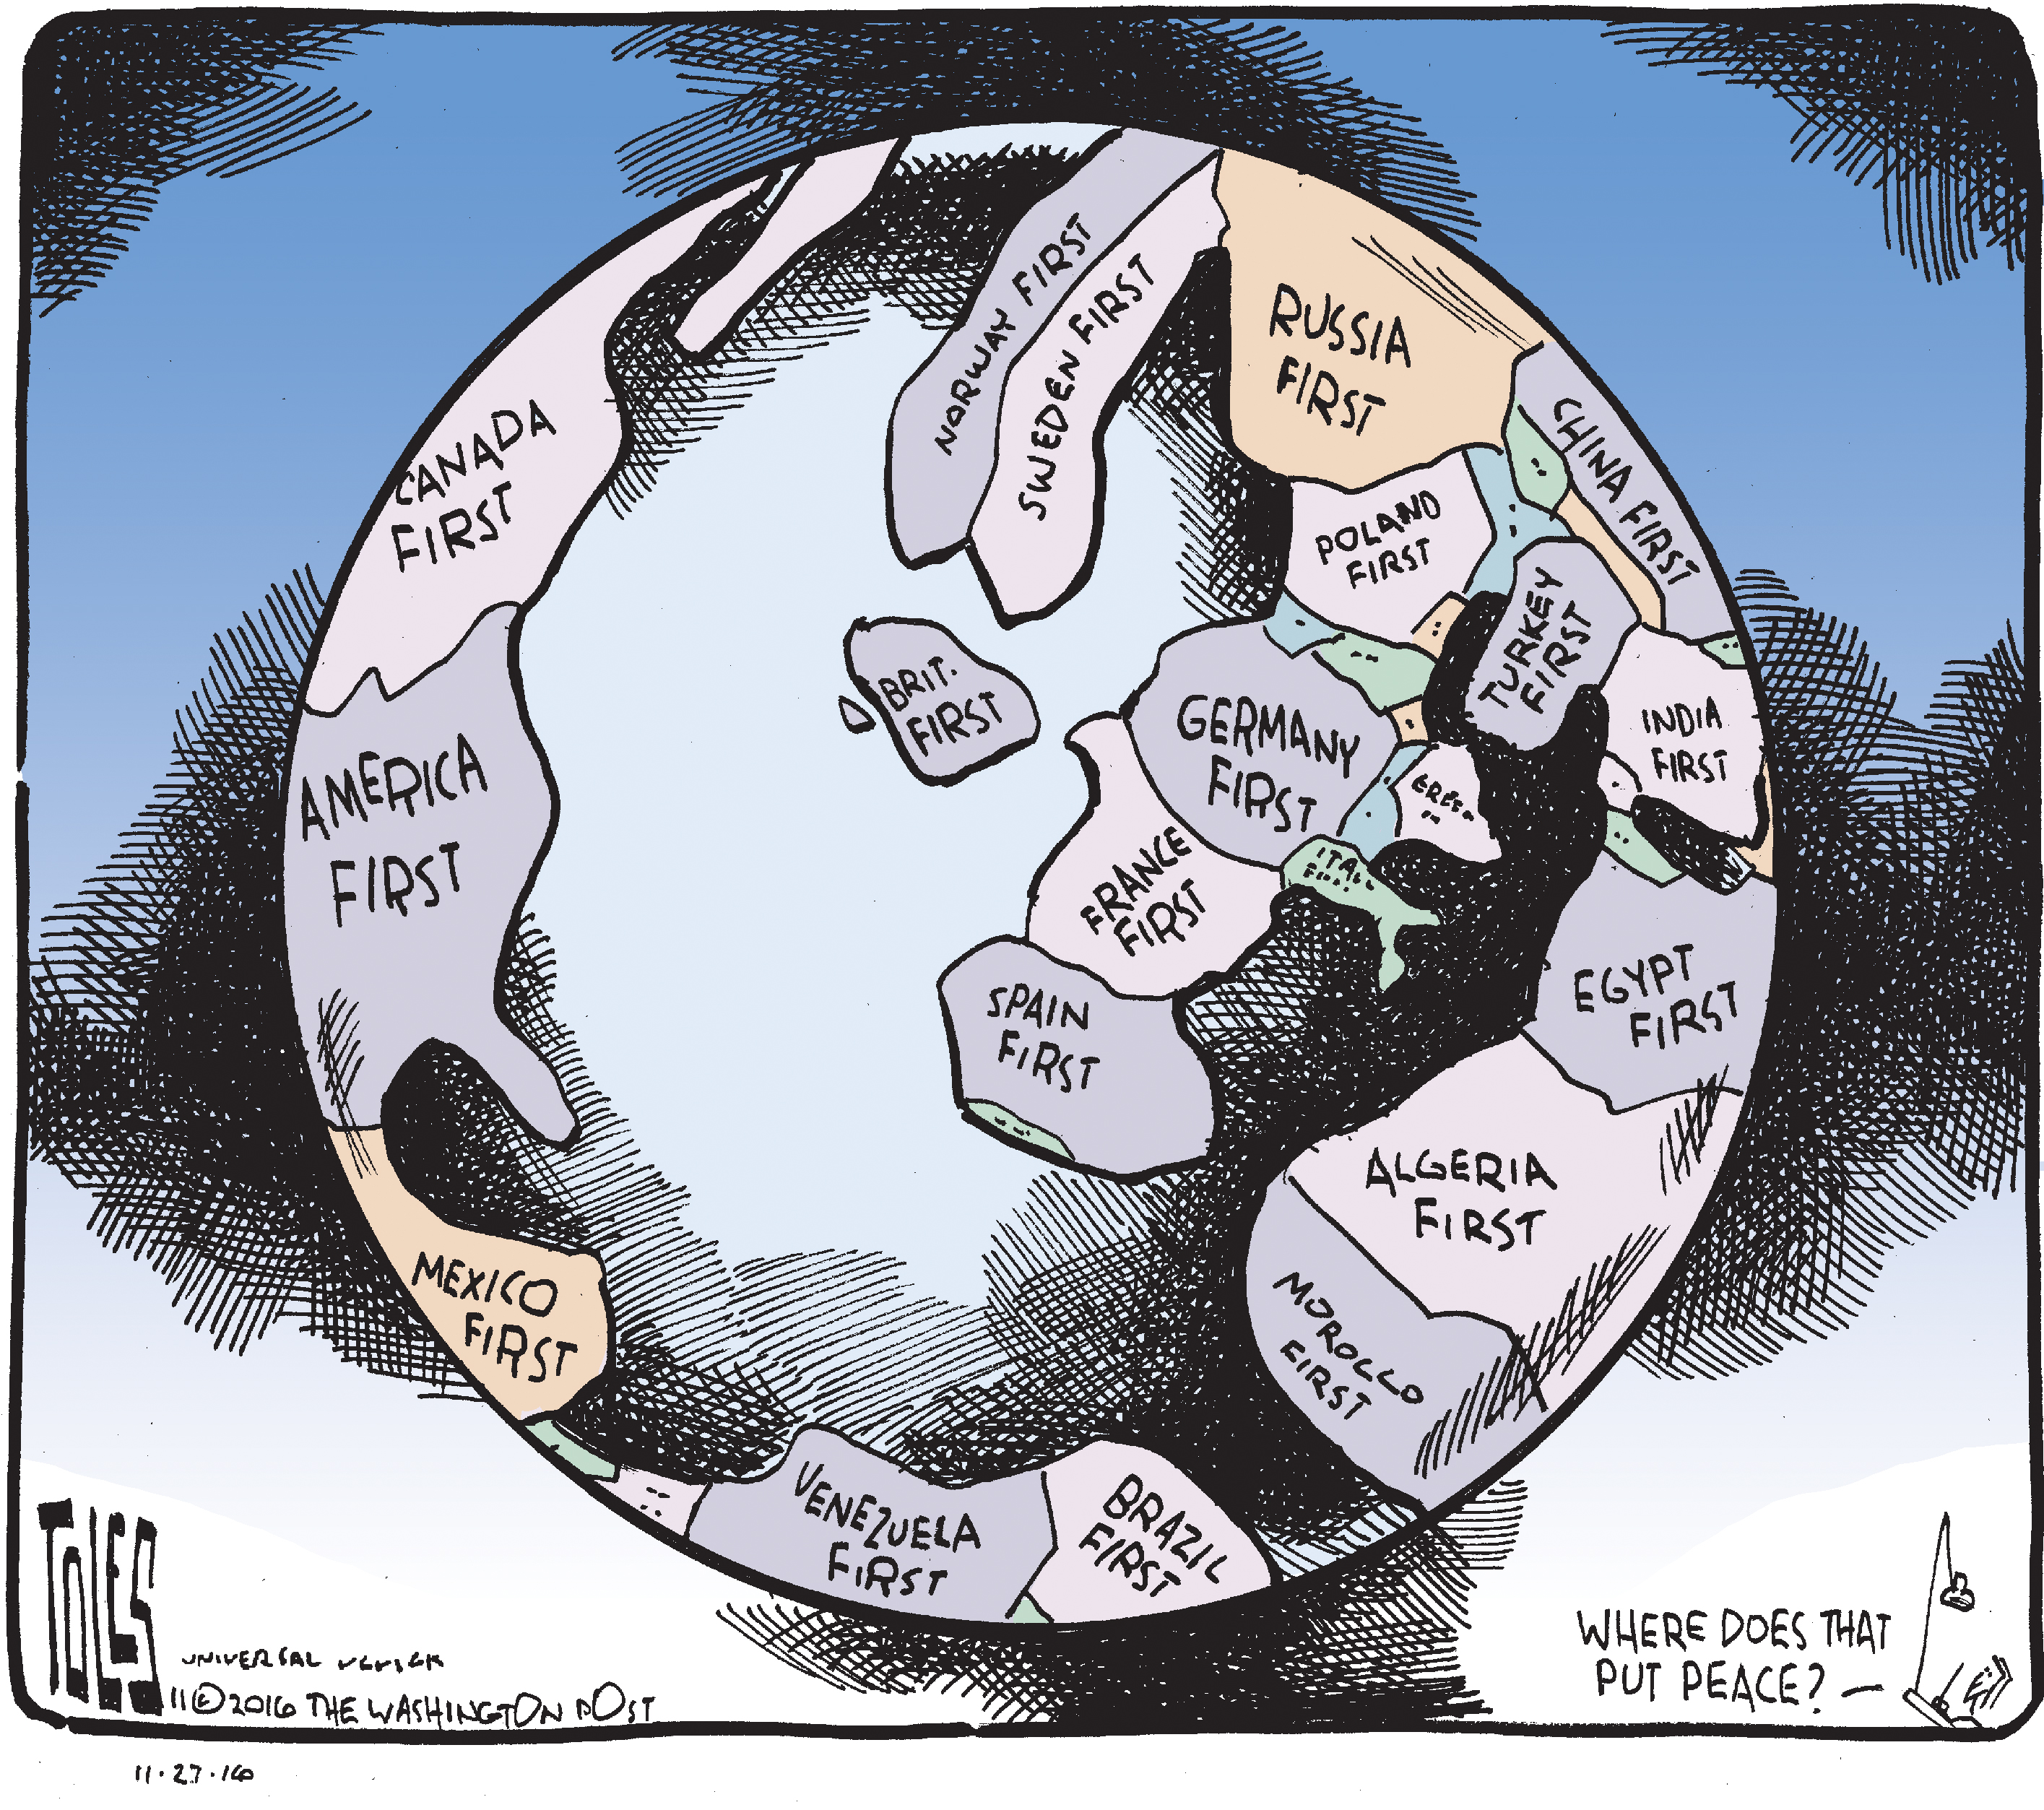
\includegraphics[width=0.3\linewidth]{Images/PopulismSatire.jpg}
    \label{F:satirapopulismo}
Come espresso dalla definizione di Gerbaudo, il populismo si afferma come il "partito piglia tutto": aggrega interessi indipendentemente dal loro grado di realizzabilità.
    \flushright
    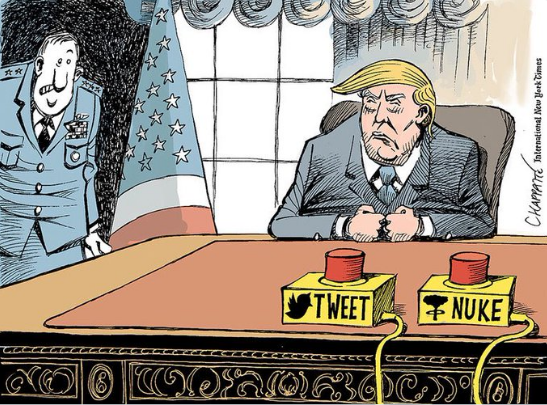
\includegraphics[width=0.3\linewidth]{Images/TrumpSatire.png}
    \label{F:satiratrump}
\end{frame}

\begin{frame}{Social Media}
    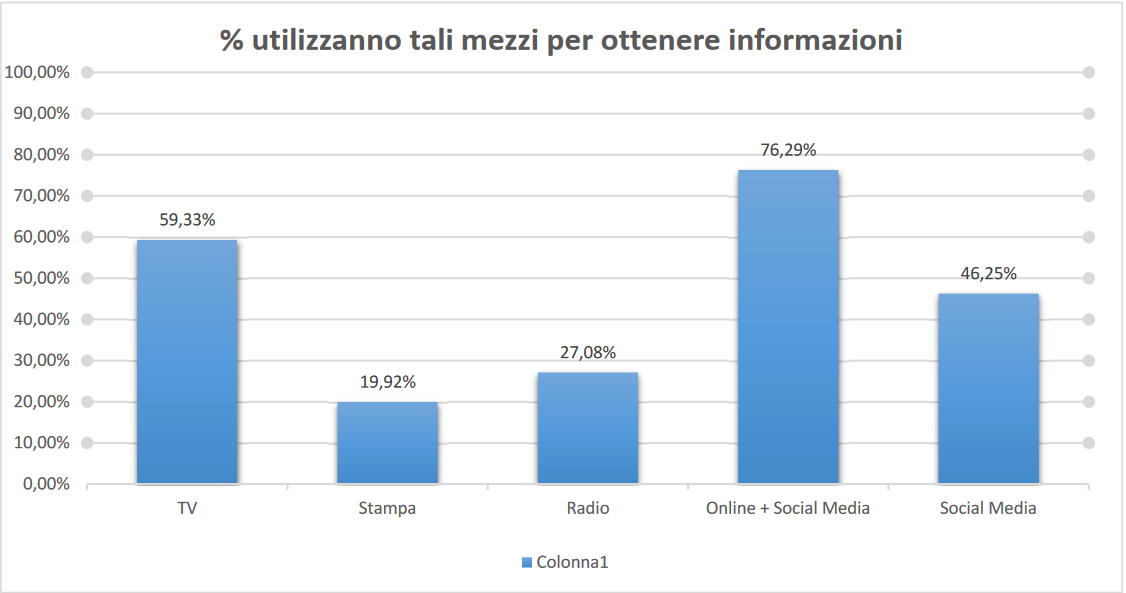
\includegraphics[width=1.0\linewidth]{Images/Screenshot 2023-10-21 at 16-17-01 graphpdf.pdf.png}
    \caption{Grafico che sintetizza le percentuali di utilizzo dei media in Europa.}
    \label{F:utilizzosocialEU}
\end{frame}

\begin{frame}
    \begin{figure}
    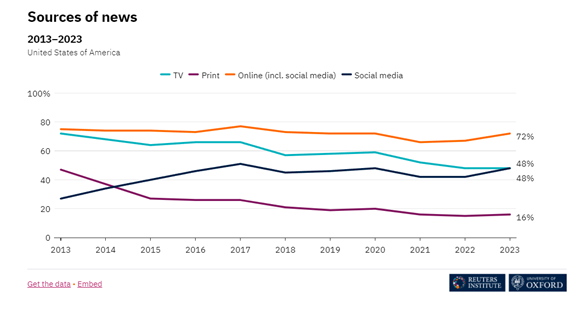
\includegraphics[width=0.7\linewidth]{Images/Sourcesofnews.png}
    \caption{Grafico che spiega l'andamento dell'utilizzo dei diversi media per l'informazione}
    \label{F:graficomezz}
    \end{figure}
\end{frame}

\begin{frame}
\begin{figure}
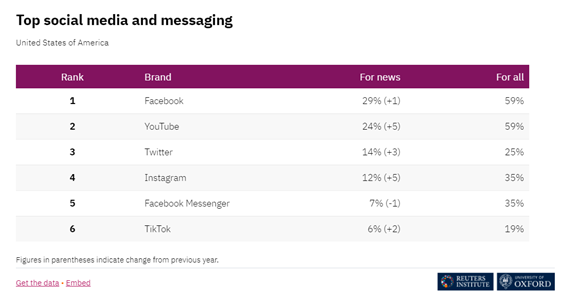
\includegraphics[width=0.6\linewidth]{Images/TopSocial.png}
    \caption{Tabella esplicativa della top 5 social in America}
    \label{F:social}
\end{figure}
\end{frame}

\bibliography{Bibliografia}
\bibliographystyle{alpha}
    
\end{document}
